% Chapter 3

\chapter{Study of Wu et. al.'s algorithm for locally optimal NAMO in unknown environments} % Main chapter title

\label{Chapter3} % For referencing the chapter elsewhere, use \ref{Chapter3}

\section{Original algorithms}\label{original_algo_section}

\paragraph{} In Wu et. al.'s proposition \parencite{wu_navigation_2010}, the basic idea is to consider either a plan that doesn't involve interacting with obstacles (which can be achieved with any pre-existing path finding algorithm), or a three-steps plan. As shown in Figure \ref{fig:Wu_Original_Algorithm-wu_components_illus}, the latter consists in, first, reaching the obstacle ($c_{1}$), second, pushing it in a single direction ($c_{2}$), and finally reaching the goal from the position we left the obstacle at ($c_{3}$).

\begin{figure}[H]
\centering
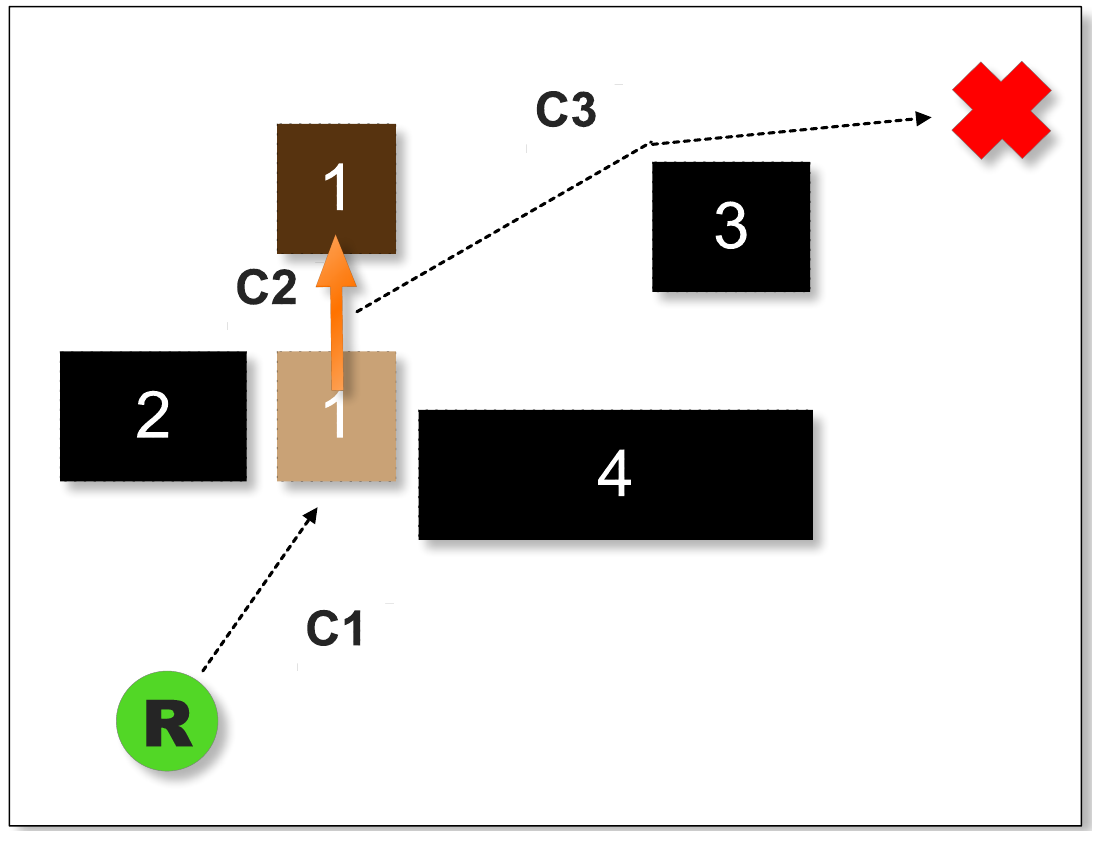
\includegraphics[width=4cm]{Figures/Wu_Original_Algorithm/wu_components_illus.png}
\caption{Figure describing the three plan components when pushing an object, as proposed in \parencite{wu_navigation_2010}.}
\label{fig:Wu_Original_Algorithm-wu_components_illus}
\end{figure}

\paragraph{} In their first article \parencite{wu_navigation_2010}, Wu et. al. describe two versions of their algorithm: a naive but locally optimal baseline one, and an optimized one, built upon the logic foundation of the first, but that loses its local optimality. Several other improvements on performance are given that restore the local optimality of the original proposition in their second article \parencite{levihn_locally_2014}. As a reminder, by locally optimal, we mean that the algorithm will \textbf{always} choose the \textbf{best} plan given its current, limited knowledge of the environment.

\paragraph{} Both algorithms assume that the robot has no prior knowledge of the environment at all, and that new information is gradually stored in a 2D metric map, assuming perfect data, and making the hypothesis that unknown space is free space. The 2D metric map is translated into a binary occupancy grid\footnote{\textbf{Occupancy grids} are used in robotics to represent the environment as a discrete grid. Binary ones represent occupied space (obstacles) by true values and free space by false ones. More complex modelizations of occupied space are also used, like associating to cells floating-point values of the probability of occupation. A more complete defition can be found here: \url{https://www.mathworks.com/help/robotics/ug/occupancy-grids.html}} for A* and the opening detection algorithm (presented in the \nameref{optimization_3} paragraph). Whereas the first proposition is limited to rectangular obstacles, the second is extended to any polygonal obstacles, and none take autonomously moving obstacles (humans, animals or animated objects) into account. In the first proposition, obstacles can only be pushed, whereas in the second one, obstacles can be translated in any direction. The considered robot is a simulated differential drive nondescript robot with a limited field of vision, that can only push obstacles in the first proposition, but can also pull them in the second one. The NAMO class of the problem is a subset of $L_1$, since a given plan can only ever imply the movement of one obstacle.

\begin{figure}[H]
\centering
\begin{subfigure}{.45\textwidth}
  \centering
  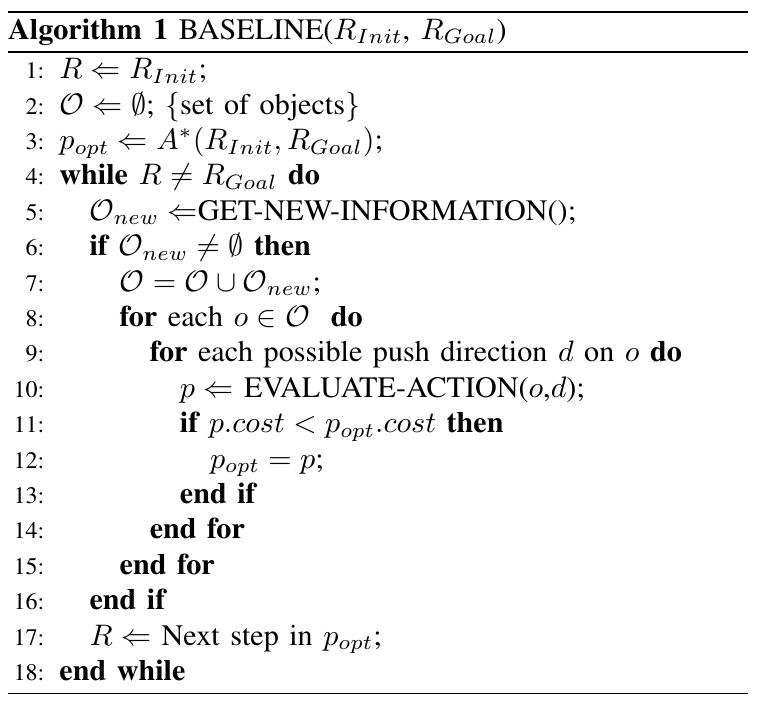
\includegraphics[width=\linewidth]{Figures/Wu_Original_Algorithm/algo1.png}
  \caption{Main loop that evaluates all plans containing the manipulation of an obstacle every time a new one is found}
  \label{fig:Wu_Original_Algorithm-algo1}
\end{subfigure}\hspace*{\fill}
\begin{subfigure}{.45\textwidth}
  \centering
  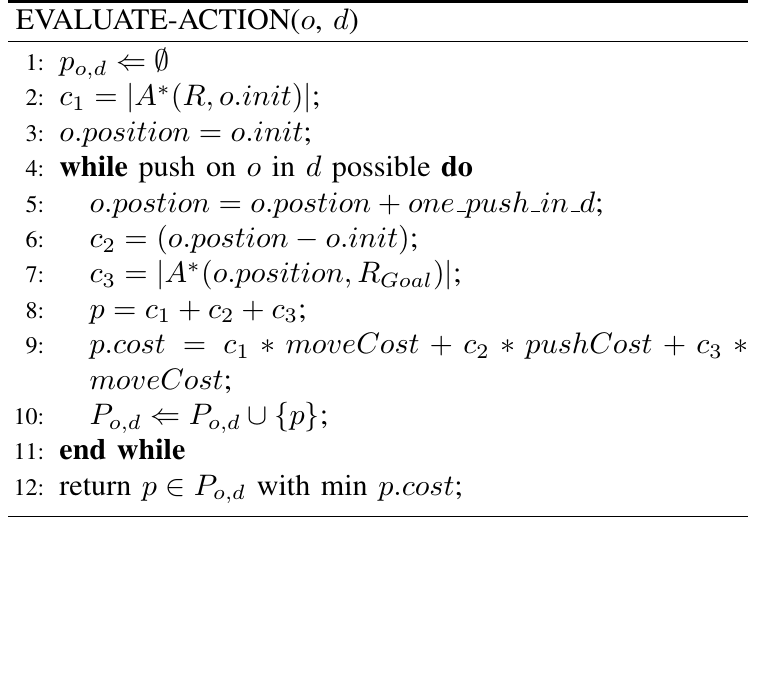
\includegraphics[width=\linewidth]{Figures/Wu_Original_Algorithm/algo2.png}
  \caption{Subroutine for evaluating all possible plans for each manipulation direction allowed on an obstacle}
  \label{fig:Wu_Original_Algorithm-algo2}
\end{subfigure}
\caption{Copy of the Baseline Algorithm proposed by Wu et. al. in \parencite{wu_navigation_2010}. The notations used are not defined in the article, hence our next section \ref{removing_ambiguity_section}, where detailed definitions can be found.}
\label{fig:Wu_Original_Algorithm-baseline}
\end{figure}

\paragraph{} The baseline algorithm is very straightforward: it uses an A* path finding subroutine to determine the optimal path between the current robot's position and the goal, avoiding all known obstacles (none at the beginning). As the robot moves forward (Figure \ref{fig:Wu_Original_Algorithm-algo1}, line 17), and therefore gains new information (same figure, line 5), whenever a new obstacle is encountered, every push action for every obstacle is re-simulated (Figure \ref{fig:Wu_Original_Algorithm-algo2}) and compared to the current optimal plan (Figure \ref{fig:Wu_Original_Algorithm-algo1}, line 11). Local optimality is guaranteed for this approach, since the A* algorithm is used with the admissible Euclidean heuristic, thus returning optimal solutions for a given state of the map and goal, and also because whenever a new obstacle is detected (= the map is in a new state), \textbf{all} possible plans are re-evaluated and compared to check if a better plan than the current one can be found or not before moving the robot again.

\paragraph{} The optimized version of the algorithm published in the first article offers four optimization steps:

\paragraph{First Optimization}\label{optimization_1} Only consider computing a new plan if the current one is actually blocked by a new obstacle (Figure \ref{fig:Wu_Original_Algorithm-algo3}, line 6). This keeps the local optimality, since a newly detected obstacle can only imply a costlier plan either moving around it or moving it (\textbf{assuming obstacles don't move by themselves, which if it were the case, could open new, better routes}): given that we can assume that the current optimal plan was optimal before the discovery of the new obstacle, we need only reconsider it if the new obstacle invalidates it.

\paragraph{Second Optimization}\label{optimization_2} Stop simulating pushes in a given direction before it becomes costlier than the current valid optimal plan, thanks to a bound (Figure \ref{fig:Wu_Original_Algorithm-algo4}, line 5). This also keeps optimality, since there are no reasons to continue evaluating actions that are already costlier than simply following the current valid optimal plan.

\begin{figure}[H]
\centering
\begin{subfigure}{.45\textwidth}
  \centering
  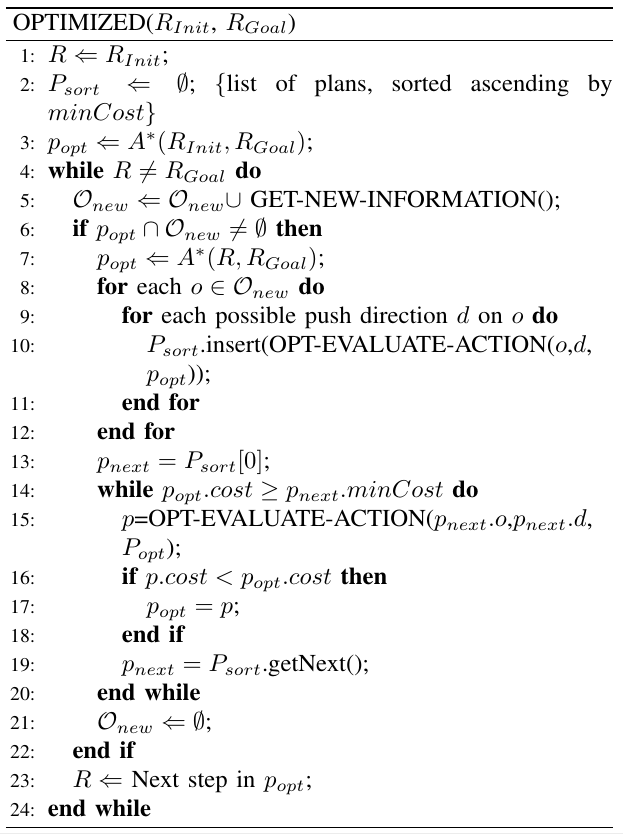
\includegraphics[width=\linewidth]{Figures/Wu_Original_Algorithm/algo3.png}
  \caption{Main loop}
  \label{fig:Wu_Original_Algorithm-algo3}
\end{subfigure}\hspace*{\fill}
\begin{subfigure}{.45\textwidth}
  \centering
  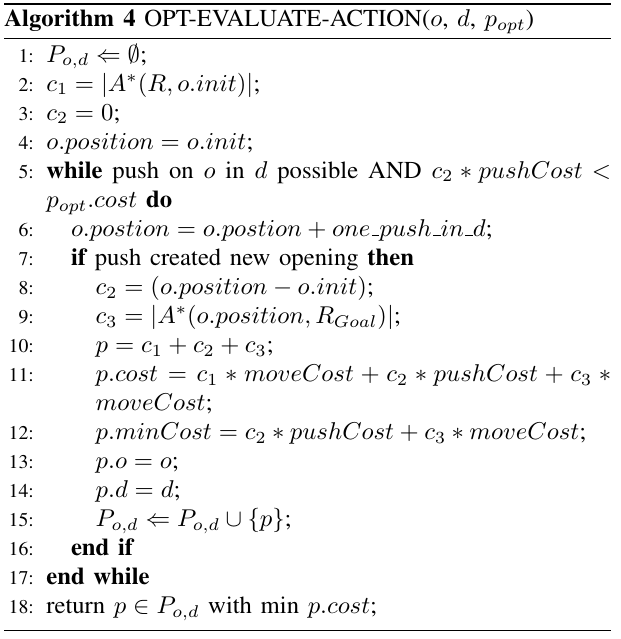
\includegraphics[width=\linewidth]{Figures/Wu_Original_Algorithm/algo4.png}
  \caption{Subroutine}
  \label{fig:Wu_Original_Algorithm-algo4}
\end{subfigure}
\caption{Copy of the Optimized Algorithm proposed by Wu et. al. in \parencite{wu_navigation_2010}.}
\label{fig:Wu_Original_Algorithm-optimized}
\end{figure}

\paragraph{Third Optimization}\label{optimization_3} Only compute the third path component (from obstacle to goal) with A* if the simulated movement actually creates an opening (Figure \ref{fig:Wu_Original_Algorithm-algo4}, line 7), since, according to the author, checking an opening creation is less computing time-consuming than running a search algorithm to the goal. The exact opening detection algorithm used is not adressed in this paper and the method used is not explicit. A technical paper later written by co-authors Levihn and Stilman \parencite{levihn_efficient_2011}, describing their new opening detection algorithm used in \parencite{levihn_locally_2014} however gives a hint at the used method: \textit{"The algorithm did not rely on search but simply observed the amount of adjacent free spaces on corners of the manipulated obstacle. While efficient, this algorithm is only applicable for world configurations populated with simple rectangular shaped static and movable obstacles. This is not realistic."}. This algorithm, like the one presented in the technical paper, only observes the variations of occupied space in the local vicinity of the movable obstacle. In the technical paper, it is explained that a new opening is detected only if the robot-diameter-inflated area of the movable obstacle is no longer intersected by the non-inflated area of another obstacle. If there are no obstacles in the robot-diameter-inflated area, then it means that the robot can pass through it, which can be considered as a local opening in the vicinity of the obstacle. This is illustrated in Figure \ref{fig:opening_detection_figures}.

\clearpage

\begin{figure}[H]

\begin{subfigure}{0.19\textwidth}
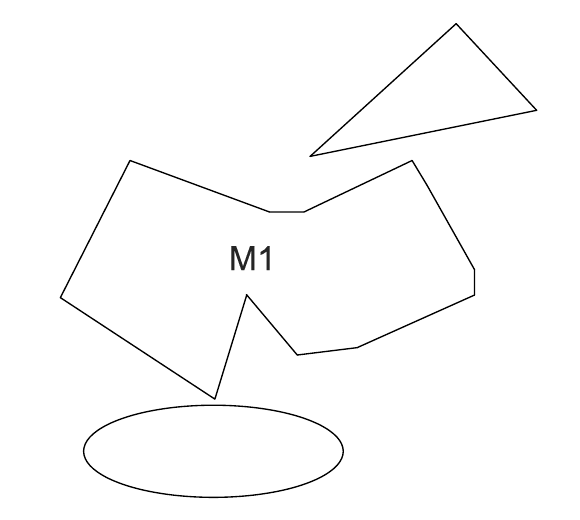
\includegraphics[width=\linewidth]{Opening_Detection/01.png}
\caption{Movable obstacle M1 and other obstacles.} \label{fig:opening_detection_01}
\end{subfigure}\hspace*{\fill}
\begin{subfigure}{0.19\textwidth}
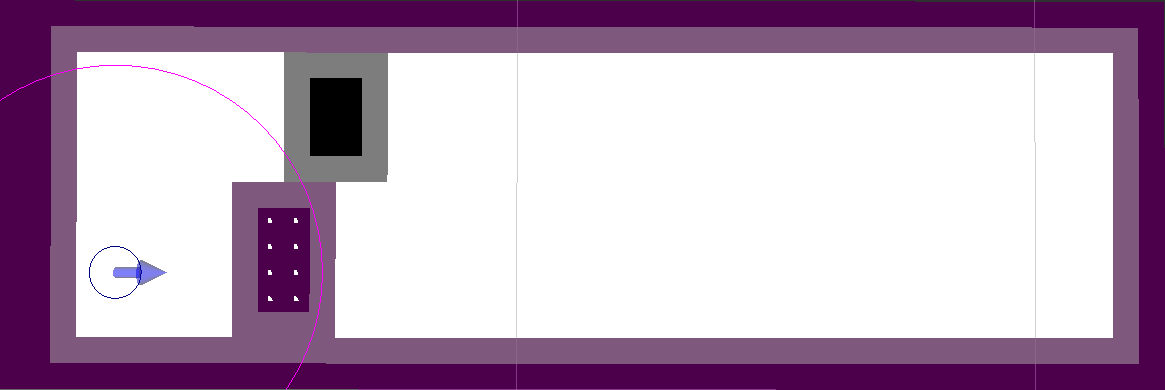
\includegraphics[width=\linewidth]{Opening_Detection/02.png}
\caption{In blue: robot-diameter-inflated movable obstacle M1. In cross-red: intersection areas with other obstacles.} \label{fig:opening_detection_02}
\end{subfigure}\hspace*{\fill}
\begin{subfigure}{0.19\textwidth}
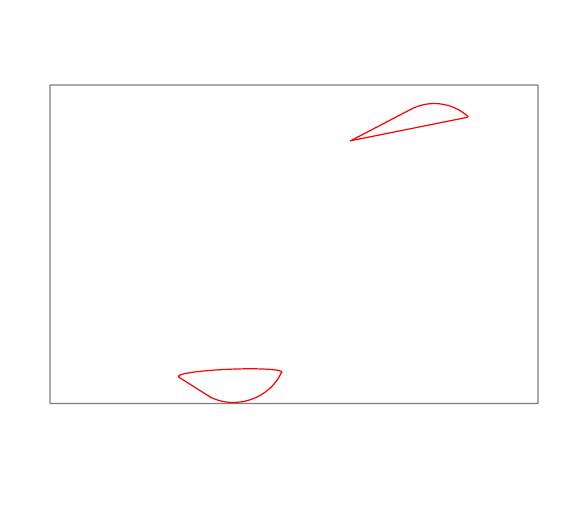
\includegraphics[width=\linewidth]{Opening_Detection/03.png}
\caption{Saved information on blocking areas before manipulation.} \label{fig:opening_detection_03}
\end{subfigure}\hspace*{\fill}
\begin{subfigure}{0.19\textwidth}
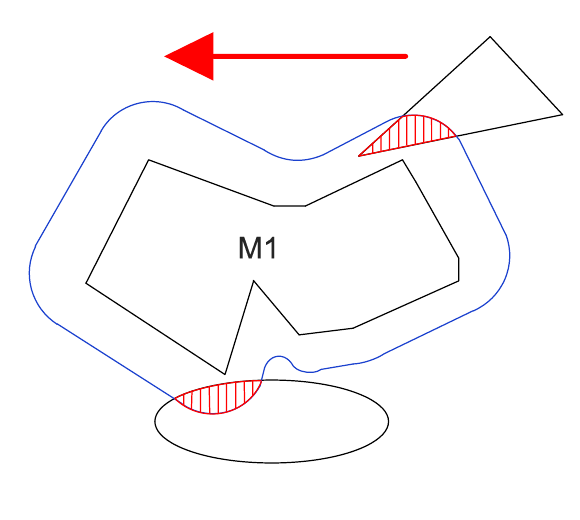
\includegraphics[width=\linewidth]{Opening_Detection/04.png}
\caption{State after M1 was translated to the left.} \label{fig:opening_detection_04}
\end{subfigure}\hspace*{\fill}
\begin{subfigure}{0.19\textwidth}
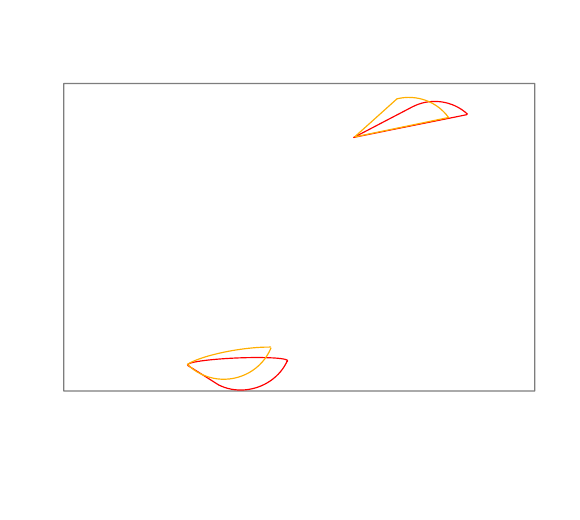
\includegraphics[width=\linewidth]{Opening_Detection/05.png}
\caption{No blocking area has disappeared: no new opening is detected.} \label{fig:opening_detection_05}
\end{subfigure}

\caption{Opening detection example given in the technical paper \parencite{levihn_efficient_2011}.}
\label{fig:opening_detection_figures}
\end{figure}

\paragraph{} However, with this definition of new opening detection, we also end up with a loss of local optimality, and also lose the algorithm's completeness. Indeed, conditioning the full evaluation of a plan by the detection of a new opening prevents from finding the solution in cases where the local environment of the obstacle does not contain any other obstacle (Figure \ref{fig:openspace_case}), or if for the considered manipulation, the local environment of the obstacle does not change (Figure \ref{fig:corridor_case}). Below are examples figures of these cases, assuming that the cost of following a path is the same whether it implies moving an obstacle or not.

\paragraph{}\label{figure_legends_paragraph} In the corridor case initial situation (Figure \ref{fig:corridor_original}), the robot (dark grey disk with a triangle) can not go to its goal (green disk with triangle) without moving the obstacle M1 (dark grey is for a movable obstacle, black is for unmovable obstacle, and light grey is for the inflation of the obstacles by the robot's radius), since the space is divided into two independent free space components (the robot's center cannot penetrate the grey or black zones without entering in collision). Furthermore, the robot can only move the obstacle by either pushing or pulling it left or right. However far the robot simulates moves in either direction, the robot-diameter-inflated area of M1 (red line) will never lose its two blocking areas (intersections between the red rectangle and the unmovable obstacle in black), therefore, no new opening will ever be detected according to the definition of the algorithm, and no plan moving the obstacle will ever be considered. However, Figure \ref{fig:corridor_optimal_path} shows clearly that a plan exists that is valid if we simply don't check for new openings (new configuration of M1, noted M1' is represented in dotted lines).

\paragraph{} In the open space case initial situation (Figure \ref{fig:openspace_original}), no new opening will ever be found however we move the obstacle, since there are no obstacles (represented in black or dark grey) in its robot-diameter-inflated area. Since, this time, there is space for the robot to move around the obstacle instead of pushing it, the algorithm will thus return this suboptimal plan, instead of the optimal one shown in Figure \ref{fig:openspace_optimal_path} that implies moving M1 to its new configuration M1'.

\begin{figure}[H]
\centering
\begin{subfigure}{.48\textwidth}
  \centering
  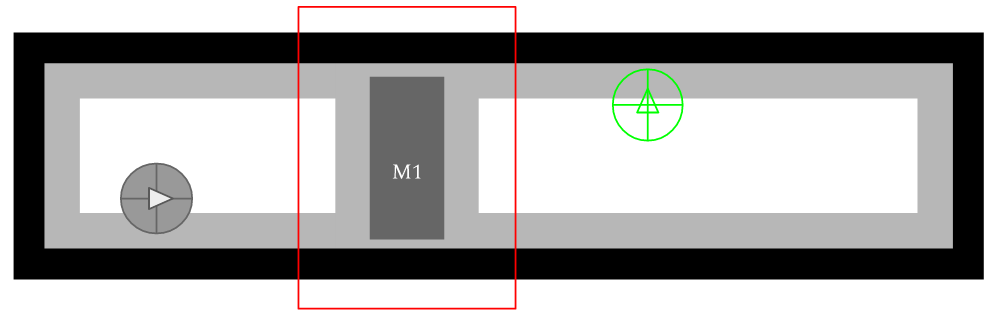
\includegraphics[width=\linewidth]{Figures/Check_New_Opening/corridor_original.png}
  \caption{Initial situation where no plan will be found when using new opening checking.}
  \label{fig:corridor_original}
\end{subfigure}\hspace*{\fill}
\begin{subfigure}{.48\textwidth}
  \centering
  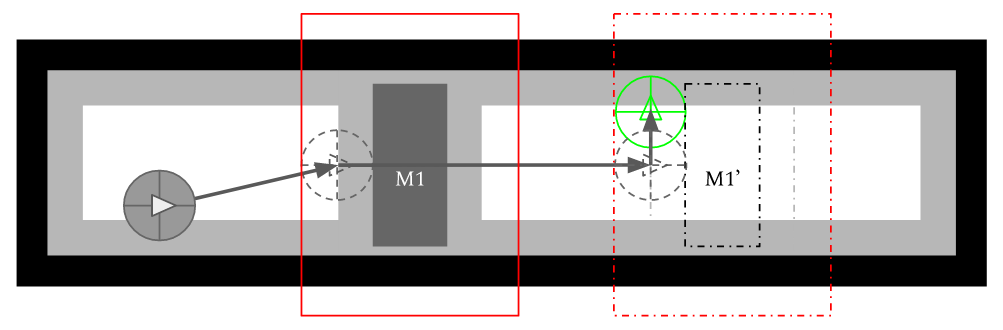
\includegraphics[width=\linewidth]{Figures/Check_New_Opening/corridor_optimal_path.png}
  \caption{Expected optimal plan.}
  \label{fig:corridor_optimal_path}
\end{subfigure}
\caption{"Corridor" case where the original algorithm will not even find a plan when it should.}
\label{fig:corridor_case}
\end{figure}

\begin{figure}[H]
\centering
\begin{subfigure}{.48\textwidth}
  \centering
  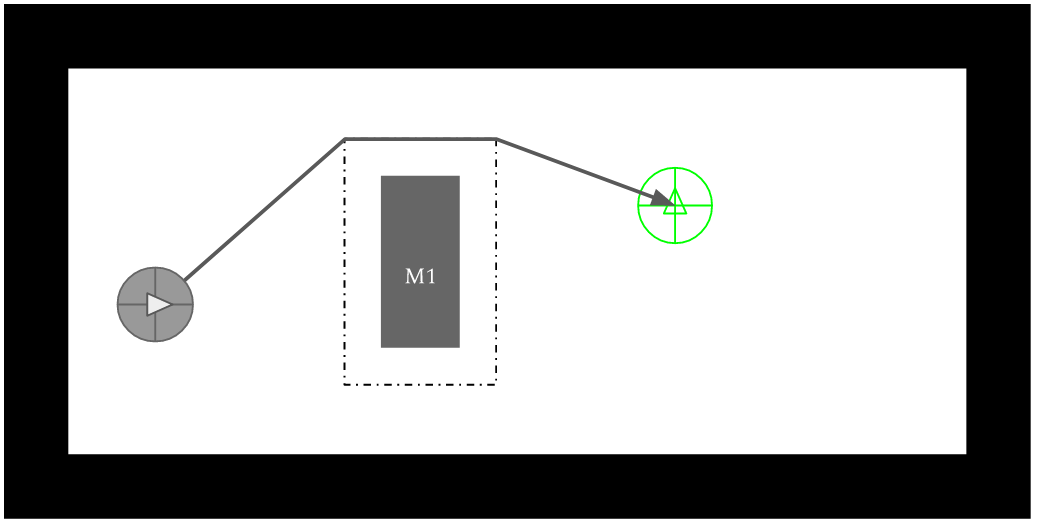
\includegraphics[width=\linewidth]{Figures/Check_New_Opening/openspace_original.png}
  \caption{Initial situation and suboptimal plan avoiding the obstacle that will be returned by the algorithm when using new opening checking.}
  \label{fig:openspace_original}
\end{subfigure}\hspace*{\fill}
\begin{subfigure}{.48\textwidth}
  \centering
  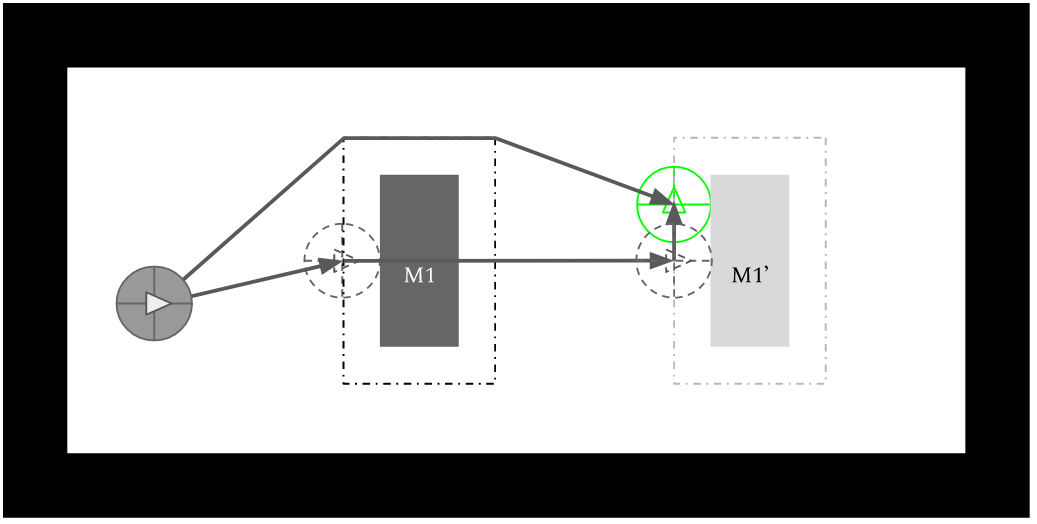
\includegraphics[width=\linewidth]{Figures/Check_New_Opening/openspace_optimal_path.png}
  \caption{Expected optimal plan is the one that pushes the obstacle.}
  \label{fig:openspace_optimal_path}
\end{subfigure}
\caption{"Open space" case where the original algorithm will only find a suboptimal plan, under the assumption that the cost of following a path is the same whether it implies moving an obstacle or not.}
\label{fig:openspace_case}
\end{figure}

\paragraph{}\label{check_opening_solution} Below, we propose, but do not provide a full demonstration for a way for restoring the optimality, assuming we are under the hypothesis of sole translations, in a single direction. Since performance is not the main focus of our work here, but optimality is, we will prefer not to use the opening check optimization step in our following algorithms propositions in chapter \ref{Chapter4}, and postpone a proof to later work.

\paragraph{} For remembrance, a new opening is never detected if:

\begin{itemize}
  \item Not a single blocking area disappears thanks to the considered manipulation, because the blocking areas do not vary enough or at all ("corridor" case, Figure \ref{fig:corridor_swept}),
  \item There are no blocking areas to begin with ("open space" case, Figure \ref{fig:openspace_swept}).
\end{itemize}

\paragraph{} In both cases, it is only interesting to consider the manipulation if it actually creates any chance of finding a plan that has a lower cost than the one that avoids the obstacle.

\paragraph{} We have an intuition that, if no new opening is detected, and if, like in the "corridor" case, no plan avoiding the obstacle was found, or, like in the "open space" case, a plan avoiding the obstacle was found, we should only consider the manipulation if it allows us to push the obstacle through the goal pose; in more precise terms, \textbf{if the goal pose is within the "inflated swept area" and the obstacle in its final position does not intersect with the goal pose}. The inflated swept area is defined as the area covered by the inflated (by the robot's radius) obstacle when moved. In the end, the overall check condition should be:

\paragraph{} \textbf{If} CHECK-NEW-OPENING($I.occGrid$, $o$, $translation$, $BA$) AND $goalPose \in$ GET-INFLATED-SWEPT-AREA($o$, $translation$, $I$) AND $goalPose \not\in o.inflatedArea$

\begin{figure}[H]
\centering
\begin{subfigure}{.48\textwidth}
  \centering
  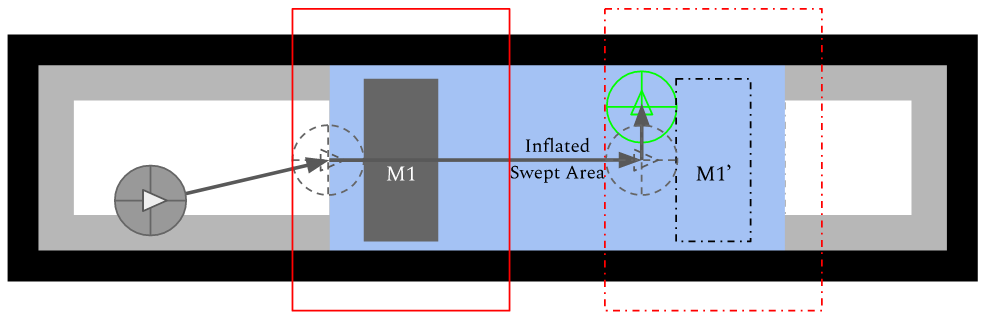
\includegraphics[width=\linewidth]{Figures/Check_New_Opening/corridor_swept.png}
  \caption{"Corridor" case: with our proposition, the optimal plan will be computed since the goal is in the blue area.}
  \label{fig:corridor_swept}
\end{subfigure}\hspace*{\fill}
\begin{subfigure}{.48\textwidth}
  \centering
  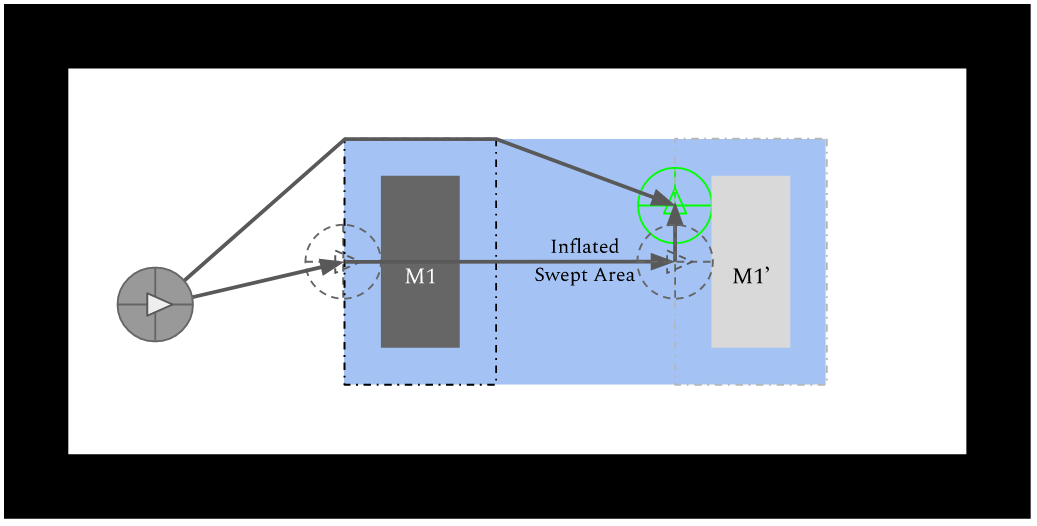
\includegraphics[width=\linewidth]{Figures/Check_New_Opening/openspace_swept.png}
  \caption{"Open space" case: again the optimal plan will be found for the same reason as in \ref{fig:corridor_swept}.}
  \label{fig:openspace_swept}
\end{subfigure}

\medskip

\begin{subfigure}{.48\textwidth}
  \centering
  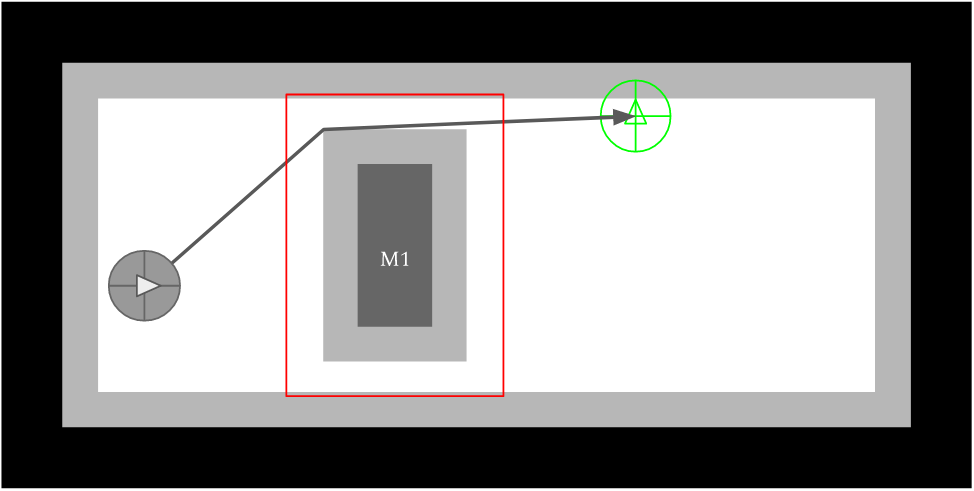
\includegraphics[width=\linewidth]{Figures/Check_New_Opening/openspace_original_offseted.png}
  \caption{"Corridor" case with goal outside the "Inflated swept area"}
  \label{fig:corridor_swept_offseted}
\end{subfigure}\hspace*{\fill}
\begin{subfigure}{.48\textwidth}
  \centering
  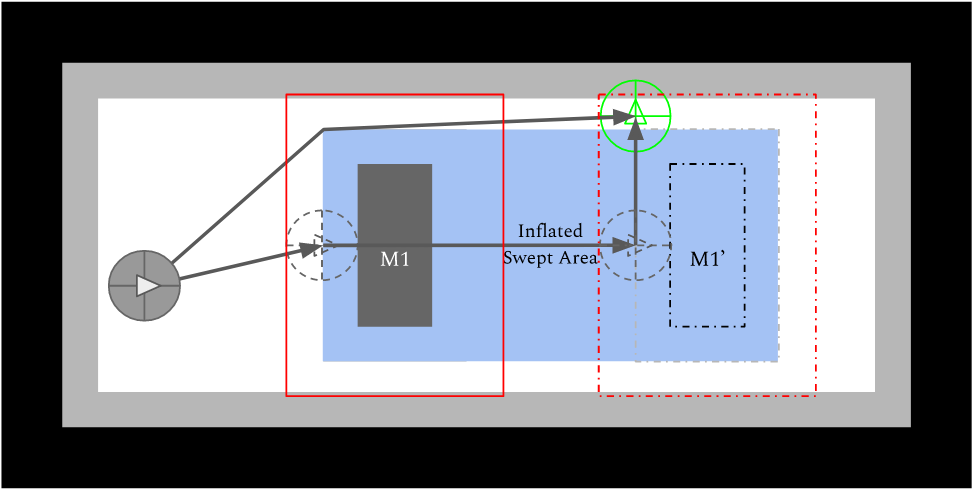
\includegraphics[width=\linewidth]{Figures/Check_New_Opening/openspace_swept_offseted.png}
  \caption{"Open space" case with goal outside the "Inflated swept area": the optimal plan is the one that avoids the obstacle: the plan moving the obstacle will never be computed since it cannot be better than the other one since the goal is not in the blue area.}
  \label{fig:openspace_swept_offseted}
\end{subfigure}

\caption{Limit cases of the original algorithm with illustration of the "Inflated swept area"} % Improve caption
\label{fig:inflated_swept_area}
\end{figure}

\paragraph{Fourth Optimization}\label{optimization_4} Finally, when the plan needs to be re-evaluated, new obstacles are evaluated first(Figure \ref{fig:Wu_Original_Algorithm-algo3}, lines 8 to 12) and the resulting paths are saved into a list (Figure \ref{fig:Wu_Original_Algorithm-algo3}, lines 2 and 10) by growing order of an underestimated heuristic cost that corresponds to sum of the costs of the plan components $c_{2}$ and $c_{3}$ (Figure \ref{fig:Wu_Original_Algorithm-algo4}, line 12). Then, this list is used to iterate over all obstacle/push direction combinations, and re-evaluate the corresponding plan (Figure \ref{fig:Wu_Original_Algorithm-algo3}, lines 13 to 20). The re-evaluation can be stopped as soon as the next pair to consider has a heuristic cost greater than the cost of the current optimal plan, improving execution performance (Figure \ref{fig:Wu_Original_Algorithm-algo4}, line 14). However, this optimization step causes the loss of the guarantee of optimality. The heuristic cost depends on $c_{2}$ and $c_{3}$, and when moving an obstacle, these components' costs may get lower. As the algorithm never updates the heuristic cost ($minCost$) in the list according to this possibility, there is therefore no guarantee that the heuristic cost will always be an underestimate. In the words of Levihn, main author of the second article:  \textit{"Second, as the algorithm does not acknowledge the fact that free-space can be created during the execution (e.g. by moving objects), which can lower c2 or c3 for some objects, this optimization steps sacrifices local optimality."} \parencite{levihn_locally_2014}

\paragraph{Note on the use of A* in the main loop} In Figure \ref{fig:Wu_Original_Algorithm-algo3}, lines 3 and 7, a call to the A* algorithm is made. For line 3, it determines the optimal path from the initial position to the goal, supposing no obstacle has been detected yet. In line 7, after the current optimal path has been invalidated by the detection of a collision between this path and a new obstacle, this call to A* star allows to get a new optimal path that avoids all obstacles that will serve as basis for the comparison with paths that consider moving obstacles.

\section{Removing ambiguity}\label{removing_ambiguity_section}

\paragraph{} The original pseudocode presented above has quite a few typos, implicit or incongruous notations that create ambiguity (e.g., storing costs and paths in the same variable, having two different variable affectation operators ($\gets$ and $=$), ...), confusing the reading. Since no pseudocode is provided by the authors for the second article's improvements propositions, it was necessary to first fix the pseudocode of the first article. The following paragraphs aim at doing this. The final pseudocode formulation is available in the Appendix section \ref{appendix_reworked_wu_section}.

\subsection{Notations and definitions}

\paragraph{Paths} are ordered sets of "steps", which are themselves robot poses.

\paragraph{A* or D* Lite} calls return A PATH as defined above. If no path is found, the returned set is empty: $\emptyset$.

\paragraph{Plans} are noted with a lowercase $p$. Lists or sets of plans will be noted with an uppercase $P$. A plan is a data structure with a "components" list attribute in which paths are stored in order of execution, and a "cost" attribute that represents the cost of executing the plan.

\paragraph{Components} of a plan are noted with a lowercase $c$.

\paragraph{The norm of a path} (written $|path|$), assuming we suppose a cost in distance,  corresponds to the sum of the euclidean distances between consecutive steps, and $+\infty$ if the path is empty.

\paragraph{The current robot pose} is noted with an uppercase $R$, the initial pose with $R_{init}$ and the goal pose with $R_{goal}$

\paragraph{Obstacles} are noted with a lowercase $o$. Lists or sets of obstacles will be noted with an uppercase $O$.

\paragraph{$moveCost$ and $pushCost$} are constants without dimension and set to 1 if we consider an optimality in distance. If we wish for optimality in energy or time, we could suppose that they would respectively represent a force or an inverse speed.

\paragraph{$one\_push\_in\_d$} is also a constant representing one elementary push. It is not explicit in the article how it is computed, but we can assume it is the multiplication of a distance constant (likely the resolution of the grid used for A*) by the unit direction vector for the given direction $d$. We will make this more explicit in our own algorithm

\paragraph{Intersection checks} between a plan and obstacles, or between obstacles, are noted with $\bigcap$ and return the set of obstacles that are intersecting, hence the line \ref{lst:line:intersection_note} in Algorithm \ref{alg:01-wu-optimized-part1}: $p_{opt} \bigcap \mathcal{O}_{new} \neq \emptyset$. In an implementation, this could be done for example by checking whether every pose in the path is not comprised in the inflated obstacles representation, and for obstacle intersection, by checking whether their polygonal representations intersect.

\paragraph{List traversal} getNext() is a helper method to traverse a list. It returns null when all elements have been traversed. Variations like getNextStep() work in the same way, at the detail that it also updates the plan's $nextStepComponent$ attribute at the same time it is called.

\paragraph{$I.withSimulatedObstacleMove$} is a notation to explicit the fact that the $c_{3}$ component must be computed assuming that the obstacle has been pushed, otherwise it does not make any sense.

\subsection{Ambiguities in the algorithm's logic}

\paragraph{Update of the robot's knowledge} The first big ambiguity in the algorithm's logic is the GET-NEW-INFORMATION method (Figure \ref{fig:Wu_Original_Algorithm-algo1}, line 5). In the original paper, it is not explicit how it works, thus we don't know how it returns a list of new obstacles. We therefore changed it into UPDATE-FROM-NEW-INFORMATION() method (Alg. \ref{alg:01-wu-optimized-part1} line \ref{lst:line:update-from-new-information_note}), that updates the world representation $I$ given in parameter, with new information about obstacles that is collected in parallel in a different execution thread. By that we mean, if this new information includes modifications to known obstacles, they are updated, and if there are new obstacles, they are added to $I$. We assume that the attribute $I.occGrid$ corresponds to the binary occupation grid with inflated obstacles in the current state, so that the path finding routine may run with it. In the same way, $I$.newObstacles corresponds to the list of newly observed obstacles since the last call of the same method (the affectation to $\mathcal{O}_{new}$ is kept as a shorter placeholder).

\paragraph{Manipulation/Push poses}\label{obstacle_pushpose_note} The second bothering ambiguity is that, for a given obstacle, the algorithm iterates over every push direction applicable to it, but doesn't iterate over every point (or manipulation/push poses) from which it could apply said push direction. We must deduce that there is an \textbf{implicit hypothesis that for a given push direction, only one point around the obstacle is a valid manipulation start point}. Therefore, we will assume that $o.init$ (Alg. \ref{alg:01-wu-optevaluateaction}, line \ref{lst:line:obstacle_pushpose_note}) corresponds to the pose the robot must get into in order to move obstacle $o$ in direction $d$. From the video\footnote{Experimentation video: \url{https://youtu.be/oQZLbJHYrl8}} that presents an implementation of the original algorithm, this pose:

\begin{itemize}
  \item Is orientated in the given direction, toward the side of the obstacle that allows to push in the given direction,
  \item Is situated on precomputed "manipulation points" that are at a robot radius distance from the side; often it seems that this point is in front of the side's middle point,
  \item Among these "manipulation points" it seems the one closest to the current position of the robot is chosen. This is fine since the algorithm seems to operate under the \textbf{implicit hypotheses that the friction between the ground and the obstacle is negligible, and that the robot's width is always smaller than the length of the obstacle's side being pushed}. Thus, if the obstacle is movable and not blocked by surrounding obstacles, it will move in the direction it is being pushed in, whatever the accessible "manipulation point" on the appropriate side may be.
\end{itemize}

\paragraph{} As the algorithm only admits pushes in straight lines, $c_{2}$ is therefore simply the set containing the initial pose for manipulation $o.init$ and the pose where the robot will stop pushing the obstacle $oSimPose$, as in line \ref{lst:line:c2_note} of Algorithm \ref{alg:01-wu-optevaluateaction}.

\paragraph{Detecting the success of a manipulation} Another ambiguity is caused by the lack of a pseudocode element translating the hypothesis given in the article that if the robot tries to move an obstacle but does not succeed, this obstacle will never be considered for manipulation again. It is meant to allow the robot to detect unmovable obstacles and to avoid an infinite loop caused by an endless evaluation of a same obstacle that cannot be moved. We translate this hypothesis in pseudocode by replacing the vague "$R \gets$ Next step in $p_{opt}$" statement (Figure \ref{fig:Wu_Original_Algorithm-algo1}, line 17) by checking whether the robot actually checking whether robot succeeded or not the desired movement by comparing the actual pose $R_{real}$ after execution and the one we wished to reach $R_{next}$ , and using the $blockedObsL$ set to remember obstacles that should never be evaluated again (Alg. \ref{alg:01-wu-optimized-part1}, lines \ref{lst:line:plan_following_note_1} to \ref{lst:line:plan_following_note_2}).

\paragraph{} Also, still in the theme of estimating the success, or rather feasibility in this case, of a manipulation, it is not said in the article how the "push on $o$ in $d$ possible" condition (Alg. \ref{alg:01-wu-optevaluateaction}, line \ref{lst:line:bound_note}) is verified. We will assume that it is only checked by verifying that the obstacle's new occupied space doesn't intersect with any other obstacle.

\paragraph{Edge cases and stop condition} In order to explicitly manage often occuring edge cases, we have added three conditions that were no originally mentioned. The first, and most important one is the stop condition in case no plan avoiding or moving obstacles has been found (Alg. \ref{alg:01-wu-optimized-part1}, line \ref{lst:line:stop_condition_note}). If no path has been found even after considering all relevant obstacles, then the algorithm must return a negative boolean value, or the goal is reached a positive one. Two conditions have been added to Algorithm \ref{alg:01-wu-optevaluateaction}, both checking if the path finding subroutine did find a path or not when computing $c_{1}$ and $c_{3}$ (lines \ref{lst:line:c1_note} and \ref{lst:line:c3_note}). For $c_{1}$, this means there is no valid plan to be found for a given obstacle and push direction. For $c_{3}$, this means there is no valid plan to be found for the given pushes in a single direction on an obstacle.

\section{Pseudocode expression of Levihn's recommendations} \label{levihn_pseudocode_section}

\paragraph{} In the second article \parencite{levihn_locally_2014}, Levihn brings alternate solutions for the \nameref{optimization_2}, \nameref{optimization_3} and \nameref{optimization_4}, reducing the computational effort and enlarging the scope of problems the algorithm can manage. For the \nameref{optimization_4}, the changes make it so optimality is no longer affected by this optimization step.

\subsection{Summary of the paper's modifications on optimizations}

\paragraph{\nameref{optimization_2}} In this article, the authors precise that they are using an improved opening detection algorithm, detailed in their separate technical paper \parencite{levihn_efficient_2011}. Since, contrary to the previous one, this new algorithm doesn't rely on obstacles being rectangles, but accepts any kind of polygon, it extends the capability of the overall algorithm to any convex polygon. The algorithm is detailed and its formulation is also improved in Appendix section \ref{appendix_eod_section}.

\paragraph{} \textbf{However, in the same way we have shown that using opening detection for considering the computation of a full plan affected optimality before (section \ref{optimization_3}), since no measures are proposed in this new article to take this into account, we must assume that local optimality is in fact not restored in this proposition}.

\paragraph{\nameref{optimization_3}} The bound that allows to reduce the number of unnecessary evaluations of extra pushes is tightened by adding to the current value of $|c_{2}|$ (computed as the product between the $pushCost$, the cost of $one\_translation\_in\_d$ and the number $seq$ of unit translations that have been simulated) the cost of the first plan component $c_{1}$ and an underestimate of the cost of the third plan component $c_{3}$ (Alg. \ref{alg:02-levihn-planforobstacle}, lines \ref{lst:line:new_bound_1} to \ref{lst:line:new_bound_2}). This underestimate is the euclidean distance between the last position of the simulated push pose $oSimPose$ and the goal pose $R_{goal}$. This bound is thus proved to be an underestimate of the real cost, keeping optimality.

\paragraph{\nameref{optimization_4}} Last but not least, a new heuristic is proposed alongside a modified version of the previous one. Basically, all obstacles that haven't been evaluated at least once are ordered in a separate list $euCostL$ by a heuristic cost that is independent from $c_{2}$ and $c_{3}$: the euclidean distance between the goal pose $R_{goal}$ and the obstacle's nearest "manipulation point" at which the robot could manipulate it. When an obstacle has been evaluated, it is added to another list $minCostL$ ordered by the usual $minCost$. Since this heuristic is more informed, $minCostL$ is used first when available (Alg. \ref{alg:02-levihn-makeplan} line \ref{lst:line:mincostl_first}). If not, $euCostL$ is used, the obstacle is re-evaluated and naturally added to the list ordered by $minCost$ (Lines \ref{lst:line:use_eucostl_1} to \ref{lst:line:use_eucostl_2}). This is achieved through the use of separate indexes for traversing the lists: $i_{e}$ and $i_{m}$. If the next entry from $minCostL$ or $euCostL$ to be considered (the one with the lowest cost) is associated with a cost that is greater than the current optimal plan, then it is not worth trying to evaluate any more options, and therefore the loop must end (Alg. \ref{alg:02-levihn-makeplan} line \ref{lst:line:stop_condition_obs_loop}). The heuristic list $minCostL$ depending on the costs of $c_{2}$ and $c_{3}$ is invalidated (emptied) anytime an obstacle has changed of place (which can potentially lower the cost of $c_{2}$ or $c_{3}$). Thus, local optimality is no longer affected. For a more detailed explanation, please consult the pseudocode (Appendix section \ref{appendix_levihn_interpretation_section}), or the original article \parencite{levihn_locally_2014}.

\paragraph{N.B on pseudocode restructuration} Since the pseudocode is our own interpretation, for easier understanding, we took the liberty of reorganizing the algorithm structure given in the original proposition of Wu \parencite{wu_navigation_2010}. We separated the plan execution and validity verification code (corresponding to lines \ref{lst:line:01_plan_execution_loop_1} to \ref{lst:line:01_plan_execution_loop_2} and \ref{lst:line:01_plan_execution_loop_3} to \ref{lst:line:01_plan_execution_loop_4} in Alg. \ref{alg:01-wu-optimized-part1}) from the code that manages the order of evaluation of obstacles (corresponding to lines \ref{lst:line:01_obstacle evaluation_loop_1} to \ref{lst:line:01_obstacle evaluation_loop_2} in Alg. \ref{alg:01-wu-optimized-part1}) into two separate methods that reflect this (Algorithm \ref{alg:02-levihn-makeandexecuteplan}: "MAKE-AND-EXECUTE-PLAN"), and (i.e Algorithm \ref{alg:02-levihn-makeplan}: "MAKE-PLAN"). We also renamed the "OPT-EVALUATE-ACTION" method (Algorithm \ref{alg:01-wu-optevaluateaction}) into "PLAN-FOR-OBSTACLE" (Algorithm \ref{alg:02-levihn-planforobstacle}) to show that our method evaluates all possibilites for a given obstacle rather than an obstacle AND a direction.

\subsection{Newly introduced notations and definitions}

\paragraph{[] operator} For the sake of readability in the pseudocode, if the list element that is asked for is out of bounds (empty list or reached end of list), the "[]" operator shall return a "fake" tuple with a null obstacle reference, and infinite cost: \{null, $+\infty$\}. This could easily be implented in code by either using a ternary operator (for example, "$minCostL[i_{m}].minCost$" would become "$minCostL[i_{m}] =$ null ? $+\infty: minCostL[i_{m}].minCost$") or implementing a custom array object with the wanted behaviour.

\paragraph{$evaluatedObstacles$} is a set that remembers which obstacles have been evaluated in the current MAKE-PLAN instance (Alg. \ref{alg:02-levihn-makeplan}, lines \ref{lst:line:evaluated_obstacles_note_1}, \ref{lst:line:evaluated_obstacles_note_2}, \ref{lst:line:evaluated_obstacles_note_3}, \ref{lst:line:evaluated_obstacles_note_4} and \ref{lst:line:evaluated_obstacles_note_5}). This is not mentioned in the original article, but it avoids evaluating an obstacle twice when it is added to $minCostL$.

\paragraph{$I$.freeSpaceCreated()} This method is used in Alg. \ref{alg:02-levihn-makeandexecuteplan}, line \ref{lst:line:second_update-from-new-information_note}, to allow the invalidation of $minCostL$ as previously explained in the Fourth Optimization paragraph. It returns True if any obstacle's occupied space has been reduced, False otherwise.

\paragraph{$I.allObstacles$} is the list of all observed obstacles in the current state (Alg. \ref{alg:02-levihn-makeandexecuteplan}, line \ref{lst:line:allobstacles}), in the same fashion as $I.newObstacles$.

\paragraph{$BA$} is a buffer for the initial blocking areas when using the new algorithm for more efficient opening detection (Alg. \ref{alg:02-levihn-planforobstacle}, lines \ref{lst:line:remember_ba_note_1} and \ref{lst:line:remember_ba_note_2}). On the first call, the variable is initialized with the initial blocking areas, and at each following call, it is passed as a parameter to reduce computational overhead. This measure is recommended by the technical paper.

\subsection{New ambiguities in the algorithm's logic}

\paragraph{} The first ambiguity in the second article \parencite{levihn_locally_2014} is that the D* Lite algorithm is mentioned instead of A*, but not even a hint of an explanation is given as to why this change, or what difference in the implementation it makes. The main feature of D* Lite being that it is designed for navigation in dynamic environments, given that no propositions are given to adapt the rest of the algorithm to dynamic environments, we will assume that no particular advantage is obtained by using D* Lite rather than A* in the proposition. Therefore, in our own proposition presented in the next chapter, we shall continue using A* as our path finding subroutine.

\paragraph{} The second ambiguity is about manipulation poses, again, as in previous section. In the article, the authors claim that \textit{"c1 only needs to be calculated once for the entire process of evaluating the current object."}. With the same reasoning as in the previous paragraph \nameref{obstacle_pushpose_note}, this affirmation can only be true if the algorithm operates under the \textbf{implicit hypothesis that for all given manipulation directions, only one point around the obstacle is considered a valid manipulation start point}. From the video \footnote{Video: \url{https://youtu.be/3AvfPVzBb-s}} accompanying the article, this point seems to be the nearest point from the robot, situated at a radius distance from the middle of a side of the obstacle. However, this hypothesis actually hinders optimality: if there is in fact a valid manipulation point for each side of the obstacle, and the algorithm knowingly doesn't consider them because they are further from the current robot's position, it will ignore the fact that a same manipulation direction could end up in opening a better path if the obstacle were moved from another manipulation point (see figures below). To guarantee optimality, we would have to simulate the manipulation in the given direction for every reachable manipulation point, thus re-evaluating $c_{1}$ for each, which would result in adding an extra "for" loop englobing the existing one.

\begin{figure}[H]
\centering
\begin{subfigure}{.35\textwidth}
  \centering
  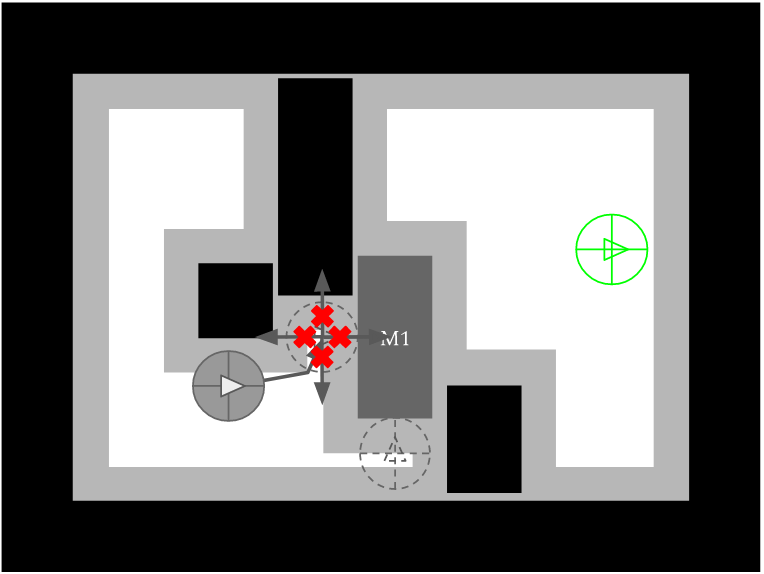
\includegraphics[width=\linewidth]{Figures/Manipulation_Pose/manip_pose_2.png}
  \caption{Nearest manipulation pose doesn't allow moving the obstacle at all (red crosses represent impossible manipulation directions).}
  \label{fig:manip_pose_2}
\end{subfigure}\hspace*{\fill}
\begin{subfigure}{.35\textwidth}
  \centering
  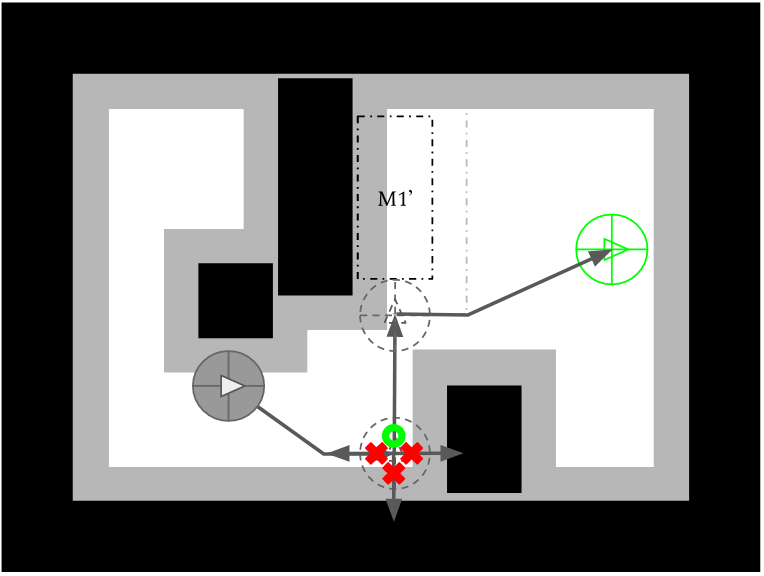
\includegraphics[width=\linewidth]{Figures/Manipulation_Pose/manip_pose_4.png}
  \caption{But if we also consider the other pose, a valid plan can be found (green circle represents possible manipulation direction).}
  \label{fig:manip_pose_4}
\end{subfigure}
\caption{Illustration of the importance of considering all possibles manipulations for all manipulation poses and not just considering the nearest one. Representations are the same as in figures \ref{fig:corridor_case} and \ref{fig:openspace_case}.}
\label{fig:manipulation_poses}
\end{figure}

\paragraph{} With all ambiguities out of the way, we now have a solid foundation on which to build upon our own proposition, with our own hypotheses: this will our focus for the next chapter.
